\section{Results}
\label{sec:results}

This section reports the controlled experiments: compression of the extended tokenizers and continued pretraining.

\subsection{Compression of repaired tokenizers}
\label{sec:compression}

Figure~\ref{fig:ksweep} sweeps the number of new merges $K$ for both models. Under the letters-only regex (\RI{}), extension saturates almost at once: for Llama-3 the first 1{,}000 merges take the premium from $2.58\times$ to $2.32\times$, and the next 63{,}000 only to $2.20\times$, within $0.01$ of the pre-token floor ($2.19\times$). For Qwen3, \RI{} cuts the premium from $4.42\times$ to $2.19\times$ by $K{=}16$k and then stops at $2.18\times$ against a floor of $2.17\times$. That \RI{} comes this close to its floor, rather than merely staying above it, is consistent with the small number of distinct Nepali pre-tokens the letters-only regex produces: the 1\,GB merge-training text has about 124k distinct pre-tokens under it, against 1.54M under the repaired regex. Under the repaired regex (\RII{}), the same merge budget keeps paying: $1.11\times$ at $K{=}16$k, $1.01\times$ at $32$k and $0.95\times$ at $64$k for both models, below parity with English and below \texttt{o200k}. At the pre-registered $K{=}32{,}000$, \RII{} encodes Nepali in 46\% of \RI{}'s tokens for both models.

All 28 extended tokenizers are lossless on the first 300 FLORES Nepali and English sentences (all 1{,}012 at $K{=}32{,}000$) and give token ids identical to the original tokenizer on all 1{,}012 English devtest sentences, as Proposition~\ref{prop:lossless} (for \RII{}) and its argument in \S\ref{sec:ceiling} (for \RI{}) require. FLORES dev, which we used to check the choice of $K$, gives the same picture within $0.02$.

\begin{figure}[t]
\centering
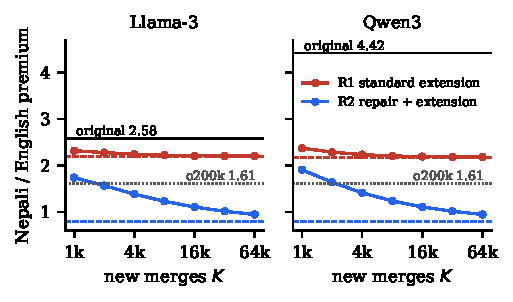
\includegraphics[width=\columnwidth]{fig_ksweep.pdf}
\caption{Nepali/English premium on FLORES-200 devtest after adding $K$ merges by continued BPE, under the letters-only regex (\RI{}) and the repaired regex (\RII{}). Dashed lines: pre-token floors of each regex, under each model's own pattern. Qwen3 tokenizers are built on Qwen3-1.7B-Base, whose tokenizer Qwen3-0.6B-Base shares. Shading: 95\% paired-bootstrap intervals.}
\label{fig:ksweep}
\end{figure}

\paragraph{Regex alone, and added tokens.} Two further arms separate the parts of \RII{}. Repairing the regex without adding merges (\RII{}, $K{=}0$) changes almost nothing: $2.61\times$ for Llama-3 (from $2.58\times$) and $4.42\times$ for Qwen3. Under the repaired regex, the old merges still tokenize Nepali words in old pieces; the regex only removes the ceiling that new merges would otherwise hit. Registering \RI{}'s new strings (31{,}999 of 32{,}000; one is a partial UTF-8 sequence) as added tokens instead of merges gives $2.35\times$ for Llama-3 and $2.19\times$ for Qwen3, no better than \RI{}. The gain of \RII{} therefore needs both the regex repair and new merges.

\paragraph{Broken syllables.} Extension under the letters-only regex makes syllable breaking worse. The share of Devanagari-bearing tokens (a slightly higher base than the all-token rate of \S\ref{sec:audit}) that begin with a combining mark rises from 57\% (Llama-3) and 33\% (Qwen3) to 67\% for both under \RI{}, because new merges can only build on mark-initial fragments. Under \RII{} it falls to 15\% and 12\%.

\paragraph{Other scripts.} We repeated the sweep for nine more languages, using the FineWeb-2 test split of each (25--361\,MB) to learn merges, with the same Devanagari-style output filter adapted to each script (Appendix~\ref{app:xling}). Table~\ref{tab:xling} (Appendix~\ref{app:xling}) gives the result at $K{=}32{,}000$; for example, \RII{} takes Tamil from $7.65\times$ to $1.02\times$ and Burmese from $11.62\times$ to $1.21\times$ on Llama-3, where \RI{} stops at $2.67\times$ and $3.02\times$. For every language written with combining marks except Thai, \RI{} stops at its floor and \RII{} reaches $0.88$--$1.24\times$. For the two scripts without combining marks, Amharic and Korean, \RI{} and \RII{} are identical at every $K$, as the mechanism predicts. All 108 extended tokenizers in this sweep are lossless and give English token ids identical to their base tokenizer on all 1{,}012 English devtest sentences.



\subsection{Continued pretraining}
\label{sec:cpt}

\begin{table*}[t]
\centering\small
\setlength{\tabcolsep}{4pt}
\begin{tabular}{lllrrrrrrrr}
\toprule
Model & Data & Arm & Tokens & ne BPB$\downarrow$ & en BPB$\downarrow$ & FLORES ne$\downarrow$ & Belebele ne & chrF ne$\to$en & chrF en$\to$ne & Gen.\ B/s \\
\midrule
Llama-3.2-1B & -- & base & 0 & 0.766 & 0.788 & 0.863 & 0.277 & 32.4 & 10.8 & 5327 \\
 & 1\,GB & \RO{} & 417M & \textbf{0.474} & 0.799 & 0.611 & 0.287 & 32.3 & 19.8 & 5147 \\
 & 1\,GB & \RI{} & 386M & 0.534 & 0.803 & 0.648 & 0.268 & 27.2 & 10.4 & 6354 \\
 & 1\,GB & \RII{} & 286M & 0.539 & 0.799 & 0.671 & 0.266 & 27.8 & 12.3 & 9398 \\
\addlinespace
 & 1\,GB + warm-up & \RO{} & 417M & 0.779 & 0.850 & 0.864 & 0.279 & 8.8 & 9.1 & 5349 \\
 & 1\,GB + warm-up & \RII{} & 286M & \textbf{0.527} & 0.840 & 0.652 & 0.283 & 16.2 & 15.4 & 11078 \\
\addlinespace
\midrule
Qwen3-0.6B & -- & base & 0 & 0.852 & 0.873 & 0.945 & 0.290 & 26.0 & 6.8 & 2186 \\
 & 1\,GB & \RO{} & 574M & \textbf{0.501} & 0.864 & 0.631 & 0.270 & 20.1 & 13.6 & 3089 \\
 & 1\,GB & \RI{} & 392M & 0.561 & 0.864 & 0.689 & 0.253 & 11.6 & 6.9 & 4972 \\
 & 1\,GB & \RII{} & 292M & 0.570 & 0.862 & 0.688 & 0.266 & 17.0 & 3.9 & 7454 \\
\addlinespace
\bottomrule
\end{tabular}
\caption{Continued pretraining on identical bytes per arm (one seed). BPB: bits per byte on held-out native text split into ${\sim}$2{,}000-byte pieces (primary metric) and on FLORES-200 devtest. Belebele: zero-shot accuracy (900 items, chance 0.25), scored on answer text. chrF++: 5-shot FLORES-200 devtest translation. Gen.\ B/s: UTF-8 bytes of Nepali generated per second (batch 64, greedy). Tokens: training tokens seen. Bold: best Nepali BPB within each block.}
\label{tab:cpt}
\end{table*}


Table~\ref{tab:cpt} reports every run. We state each comparison with the pre-registered paired bootstrap over held-out Nepali pieces (difference in bits per byte, 95\% interval).

\paragraph{Extension of either kind costs quality at this budget.} For both models, continued pretraining without new tokens (\RO{}) gives the lowest held-out Nepali BPB: 0.474 for Llama-3.2-1B (from 0.766) and 0.501 for Qwen3-0.6B (from 0.852). Both extended arms end higher, by similar amounts: \RI{} by $+0.060$ $[+0.059, +0.061]$ (Llama) and $+0.060$ $[+0.059, +0.061]$ (Qwen), \RII{} by $+0.066$ $[+0.065, +0.067]$ and $+0.070$ $[+0.068, +0.071]$ bits per byte. The cost therefore does not come mainly from the repair: it is almost as large ($+0.060$ against $+0.066$ and $+0.070$) when 32{,}000 tokens are added under the original regex. The new rows start from averages of existing rows; with 1\,GB of Nepali they do not catch up with the original vocabulary, which the base model already knows. \RO{} is also best at English-to-Nepali translation on both models.

\paragraph{Among extensions, the repair is close to standard extension and much cheaper.} \RII{} minus \RI{} on Nepali is $+0.0058$ $[+0.0049, +0.0067]$ bits per byte for Llama, inside the pre-registered non-inferiority margin of 0.01, and $+0.0094$ $[+0.0086, +0.0101]$ for Qwen, whose upper bound exceeds the margin by $0.0001$; under the pre-registered rule of amendment 2, \RII{} is non-inferior to \RI{} on Llama, and non-inferiority is not shown on Qwen, where the interval lies entirely above zero. On FLORES devtest the two are tied for Qwen (0.689 and 0.688). \RII{} reaches these numbers with 26\% (Llama) and 26\% (Qwen) fewer training tokens than \RI{}, is better on English for both models ($-0.003$ and $-0.002$, intervals excluding zero), and generates Nepali 1.48$\times$ (Llama) and 1.50$\times$ (Qwen) faster than \RI{}, and 1.83$\times$ and 2.41$\times$ faster than \RO{}, because each token carries more text. When \RI{} is stopped after the same number of steps as \RII{} and both are scored on the same 1\,MB of held-out Nepali, \RII{} is $+0.0056$ $[+0.0038, +0.0075]$ bits per byte worse for Llama and tied for Qwen ($+0.0000$ $[-0.0015, +0.0015]$); \RI{}'s learning rate has not annealed at that point.
%% EXPB-RESULTS

\paragraph{English is unaffected.} The registered English control holds: \RII{} minus \RO{} on held-out English is $+0.0003$ $[-0.0001, +0.0007]$ bits per byte for Llama (non-inferior) and $-0.0028$ $[-0.0031, -0.0025]$ for Qwen (better), as the invariance result predicts for the tokenizer and the equal English data in every arm predicts for the model.

